\documentclass[11pt,a4paper]{article}
\usepackage[T1]{fontenc}\usepackage{lmodern}
\usepackage[margin=22mm,headheight=14pt]{geometry}
\usepackage{amsmath,amssymb,bm,booktabs,tabularx,array,graphicx,float,fancyhdr,microtype,xcolor}
\usepackage[colorlinks=true,linkcolor=blue!45!black,urlcolor=blue!45!black,citecolor=blue!45!black]{hyperref}
\setlength{\parindent}{0pt}\setlength{\parskip}{5pt}\renewcommand{\arraystretch}{1.15}
\pagestyle{fancy}\fancyhf{}\fancyhead[L]{\small QFT Project B | Step 3}\fancyhead[R]{\small Group B}\fancyfoot[C]{\thepage}
\newcommand{\dd}{\mathrm{d}}
\begin{document}\hypersetup{pageanchor=false}
\begin{titlepage}\centering\vspace*{3mm}

\includegraphics[width=36mm]{assets/bits_logo.png}\par\vspace{13mm}
{\Large\bfseries BITS PILANI K.K. BIRLA GOA CAMPUS\par}\vspace{3mm}
{\large\bfseries Department of Physics\par}\vspace{18mm}
{\LARGE\bfseries What Quantum Trace Can\\[2mm] a Heavy Particle Leave?\par}\vspace{6mm}
{\large Curvature--Spectator Entanglement\\and the Cosmological Collider\par}\vspace{10mm}
{\large\bfseries Step 3: Canonical Equations\par}\vspace{17mm}
{\Large\bfseries Group-B\par}\vspace{5mm}
\begin{tabular}{ll}Priyansh Rawat & 2023B5A70968G\\Mayank Sinha & 2023B5A70942G\\Samarth Bhatnagar & 2023B5A70853G\end{tabular}
\vfill{\large Under Professor: Rudranil Basu\par}\vspace{7mm}{29 October 2026\par}
\end{titlepage}\setcounter{page}{1}\hypersetup{pageanchor=true}
\section{Legendre transform with derivative mixing}
For one real Fourier sector,
\begin{equation}L_k=\frac{a^2}{2}(q'^2+\sigma'^2)-\frac{a^2k^2}{2}(q^2+\sigma^2)-\frac{a^4m^2}{2}\sigma^2+a^3\rho q'\sigma.\end{equation}
Differentiating the Lagrangian, rather than identifying momenta from the unmixed theory, gives
\begin{equation}\pi_q=a^2q'+a^3\rho\sigma,\qquad\pi_\sigma=a^2\sigma'.\end{equation}
Hence $q'=(\pi_q-a^3\rho\sigma)/a^2$ and $\sigma'=\pi_\sigma/a^2$. Substituting these velocities into $H_k=\pi_q q'+\pi_\sigma\sigma'-L_k$ yields
\begin{equation}\boxed{H_k=\frac{(\pi_q-a^3\rho\sigma)^2+\pi_\sigma^2}{2a^2}+\frac{a^2k^2}{2}(q^2+\sigma^2)+\frac{a^4m^2}{2}\sigma^2.}\end{equation}
The square contains $a^4\rho^2\sigma^2/2$. Dropping it changes the dynamics even though the mixing in $L_k$ is linear in $\rho$. A symbolic calculation independently expands the Legendre transform and verifies exact equality with this Hamiltonian.
Hamilton's equations are
\begin{align}q'&=(\pi_q-a^3\rho\sigma)/a^2,&\pi_q'&=-a^2k^2q,\\ \sigma'&=\pi_\sigma/a^2,&\pi_\sigma'&=a\rho\pi_q-a^2k^2\sigma-a^4(m^2+\rho^2)\sigma.\end{align}
They also fix the initial velocity of a spectator-only column: an initially vanishing $\pi_q$ implies a nonzero $q'$ when $\sigma\ne0$.

\newpage
\section{Dimensionless equations and an independent formulation}
Set $x=-k\eta$, $M=m/H$, $g=\rho/H$, and write the two independent mode columns as $q_k^a=Hk^{-3/2}Q_a$, $\sigma_k^a=Hk^{-3/2}\Sigma_a$. The canonical equations are
\begin{align}\partial_xQ&=g\Sigma/x-x^2\Pi_q,&\partial_x\Pi_q&=Q/x^2,\\\partial_x\Sigma&=-x^2\Pi_\sigma,&\partial_x\Pi_\sigma&=\Sigma/x^2+(M^2+g^2)\Sigma/x^4-g\Pi_q/x.\end{align}
For $N=-\ln x$, $\partial_N=-x\partial_x$. Eliminating momenta gives the independently implemented velocity equations
\begin{align}\ddot Q+3\dot Q+x^2Q&=-g(\dot\Sigma+3\Sigma),\\\ddot\Sigma+3\dot\Sigma+(x^2+M^2)\Sigma&=g\dot Q,\\\Pi_q&=(\dot Q+g\Sigma)/x^3,\qquad\Pi_\sigma=\dot\Sigma/x^3.\end{align}
Both implementations evolve two complex columns, preserving the phases needed later. At $M=2$, $g=0.1$, $X=100$, $x_f=10^{-3}$, DOP853 with relative/absolute tolerances $10^{-10}/10^{-12}$ gives a maximum scaled column difference of $2.010\times10^{-7}$ and an entropy difference of $5.111\times10^{-7}$. The scaled difference is $|u_N-u_x|/(1+|u_N|)$; it remains meaningful near a zero of a mode column. Production precision and initial-state tests are established in the next steps.
\begin{figure}[H]\centering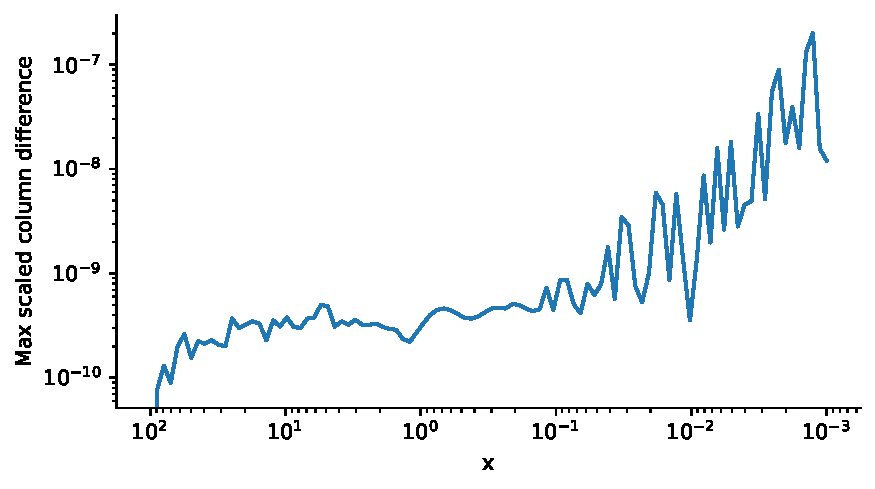
\includegraphics[width=.91\linewidth]{figures/formulation_agreement.pdf}\caption{Agreement of canonical and velocity evolutions on identical finite-time initial data. The comparison is made before any covariance normalisation.}\end{figure}
\textbf{Code and supporting data:} \href{https://github.com/rawatpriyansh17/QFT-PROJECT-GROUP-B/tree/main/step3}{step3 on GitHub}.\newpage\section*{Contributions (equal)}\begin{center}\begin{tabularx}{\linewidth}{p{33mm}X}\toprule Member & Contribution\\\midrule Priyansh Rawat & Legendre transform and Hamiltonian derivation.\\[3mm]Samarth Bhatnagar & Dimensionless and velocity equations; convention checks.\\[3mm]Mayank Sinha & Independent numerical formulations and agreement tests.\\\bottomrule\end{tabularx}\end{center}\end{document}